\chapter{Diseño del sistema propuesto}
\label{chapter:disenio}

\chapquote{Si tienes tanto miedo al fracaso, nunca tendrás éxito. Tienes que arriesgarte.}{Mario Andretti}

\section{Descripción del caso de estudio} \label{section:CasoEstudio}


\section{Diseño del sistema}

    \subsection{Casos de uso}
    \subsection{Diagramas de secuencia}
    \subsection{Interfaz de usuario}

\section{Buffer}

\subsection{Casos de uso}

    \subsubsection{Caso de uso 1: Extracción de datos de un \gls{wearable}}


    \begin{table}[h]
        \centering
        \begin{tabularx}{\textwidth}{|c|X|X|}
            \hline
            Evento activador & \multicolumn{2}{|c|}{X} \\
            \hline
            Actor primario & \multicolumn{2}{|c|}{X} \\
            \hline
            Precondición & \multicolumn{2}{|c|}{X} \\
            \hline
            \multirow{2}{*}{Flujo normal} & Paso & Acción \\
            \cline{2-3} & X & I'have been waiting for the weekend to begin \\
            \hline
            \multirow{2}{*}{Flujo alternativo} & Paso & Acción \\
            \cline{2-3} & I'have been waiting for the weekend to begin & X \\
            \hline
            Postcondición & \multicolumn{2}{|c|}{X} \\
            \hline
            \multirow{2}{*}{Excepciones}  & Paso & Acción \\
            \cline{2-3} & X & X \\
            \hline
        \end{tabularx}
        \caption{Especificación del caso de uso 1: Extracción de datos de un \gls{wearable}}
        \label{tabla:caso_uso_1}
    \end{table}
    
    \subsubsection{Caso de uso 2: Seguimiento individual}

    \begin{table}[h]
        \centering
        \begin{tabularx}{\textwidth}{|c|X|X|}
            \hline
            Evento activador & \multicolumn{2}{|c|}{X} \\
            \hline
            Actor primario & \multicolumn{2}{|c|}{X} \\
            \hline
            Precondición & \multicolumn{2}{|c|}{X} \\
            \hline
            \multirow{2}{*}{Flujo normal} & Paso & Acción \\
            \cline{2-3} & X & I'have been waiting for the weekend to begin \\
            \hline
            \multirow{2}{*}{Flujo alternativo} & Paso & Acción \\
            \cline{2-3} & I'have been waiting for the weekend to begin & X \\
            \hline
            Postcondición & \multicolumn{2}{|c|}{X} \\
            \hline
            \multirow{2}{*}{Excepciones}  & Paso & Acción \\
            \cline{2-3} & X & X \\
            \hline
        \end{tabularx}
        \caption{Especificación del caso de uso 2: Seguimiento individual}
        \label{tabla:caso_uso_2}
    \end{table}
    
    \subsubsection{Caso de uso 3: Seguimiento conjunto}

    \begin{table}[h]
        \centering
        \begin{tabularx}{\textwidth}{|c|X|X|}
            \hline
            Evento activador & \multicolumn{2}{|c|}{X} \\
            \hline
            Actor primario & \multicolumn{2}{|c|}{X} \\
            \hline
            Precondición & \multicolumn{2}{|c|}{X} \\
            \hline
            \multirow{2}{*}{Flujo normal} & Paso & Acción \\
            \cline{2-3} & X & I'have been waiting for the weekend to begin \\
            \hline
            \multirow{2}{*}{Flujo alternativo} & Paso & Acción \\
            \cline{2-3} & I'have been waiting for the weekend to begin & X \\
            \hline
            Postcondición & \multicolumn{2}{|c|}{X} \\
            \hline
            \multirow{2}{*}{Excepciones}  & Paso & Acción \\
            \cline{2-3} & X & X \\
            \hline
        \end{tabularx}
        \caption{Especificación del caso de uso 3: Seguimiento conjunto}
        \label{tabla:caso_uso_3}
    \end{table}
    
    \subsubsection{Caso de uso 4: Recopilación del histórico?}

    \begin{table}[h]
        \centering
        \begin{tabularx}{\textwidth}{|c|X|X|}
            \hline
            Evento activador & \multicolumn{2}{|c|}{X} \\
            \hline
            Actor primario & \multicolumn{2}{|c|}{X} \\
            \hline
            Precondición & \multicolumn{2}{|c|}{X} \\
            \hline
            \multirow{2}{*}{Flujo normal} & Paso & Acción \\
            \cline{2-3} & X & I'have been waiting for the weekend to begin \\
            \hline
            \multirow{2}{*}{Flujo alternativo} & Paso & Acción \\
            \cline{2-3} & I'have been waiting for the weekend to begin & X \\
            \hline
            Postcondición & \multicolumn{2}{|c|}{X} \\
            \hline
            \multirow{2}{*}{Excepciones}  & Paso & Acción \\
            \cline{2-3} & X & X \\
            \hline
        \end{tabularx}
        \caption{Especificación del caso de uso 4: Recopilación del histórico?}
        \label{tabla:caso_uso_4}
    \end{table}

\subsection{Diagramas de secuencia}

    \subsubsection{Diagramas de secuencia 1: Extracción de datos de un \gls{wearable}}
        La secuencia lógica de la extracción de datos de un \gls{wearable} es la siguiente (Figura X):

        \begin{enumerate}
            \item Hola
            \item Mundo
            \item Bifurcación
            \begin{enumerate}
                \item Primario
                \item Alternativo
            \end{enumerate}
        \end{enumerate}
    
    \subsubsection{Diagramas de secuencia 2: Seguimiento individual}
        La secuencia lógica del seguimiento individual es la siguiente (Figura X):

        \begin{enumerate}
            \item Hola
            \item Mundo
            \item Bifurcación
            \begin{enumerate}
                \item Primario
                \item Alternativo
            \end{enumerate}
        \end{enumerate}
    
    \subsubsection{Diagramas de secuencia 3: Seguimiento conjunto}
        La secuencia lógica del seguimiento conjunto es la siguiente (Figura X):

        \begin{enumerate}
            \item Hola
            \item Mundo
            \item Bifurcación
            \begin{enumerate}
                \item Primario
                \item Alternativo
            \end{enumerate}
        \end{enumerate}
        
    \subsubsection{Diagramas de secuencia 4: Recopilación del histórico?}
        La secuencia lógica de la recopilación del histórico es la siguiente (Figura X):

        \begin{enumerate}
            \item Hola
            \item Mundo
            \item Bifurcación
            \begin{enumerate}
                \item Primario
                \item Alternativo
            \end{enumerate}
        \end{enumerate}

    \subsubsection{[WIP] Diagramas de secuencia 5: Post cuestionario}
        La secuencia lógica de la recopilación del histórico es la siguiente (Figura X):

        \begin{enumerate}
            \item Android invoca a la tarea \textit{Upload}
            \item Se comprobará si hay datos de estrés pendientes de enviar.
            \item Si hay datos pendientes de est
            \item Bifurcación
            \begin{enumerate}
                \item Primario
                \item Alternativo
            \end{enumerate}
        \end{enumerate}

Diagrama ER

\begin{sidewaysfigure}[h]
    \centering
    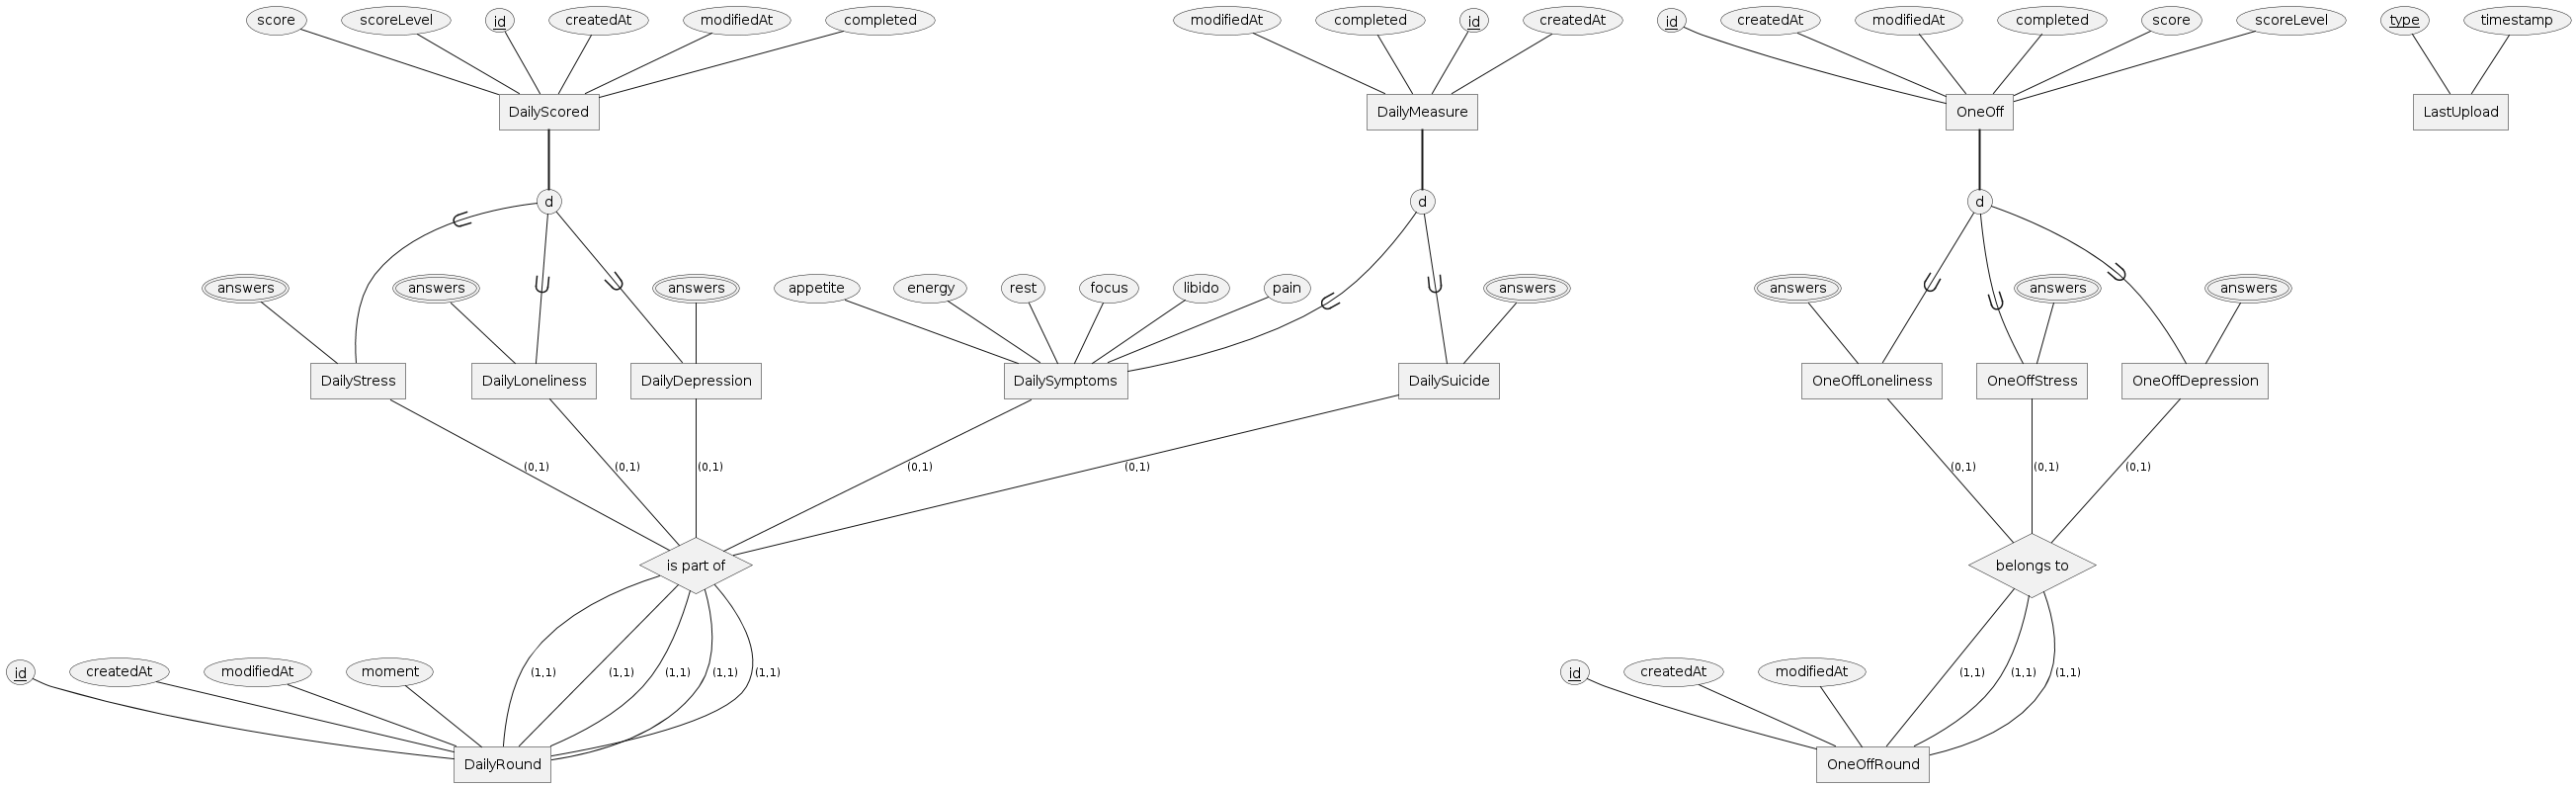
\includegraphics[width=1\textwidth]{figures/bd/ER simple.png}
    \caption[Diagrama ER]{Diagrama ER. Elaboración propia}
    \label{figure:disenio:diagrama_er}
\end{sidewaysfigure}

Diagrama colección datos usuario (\textit{user data})

\begin{figure}[h]
    \centering
    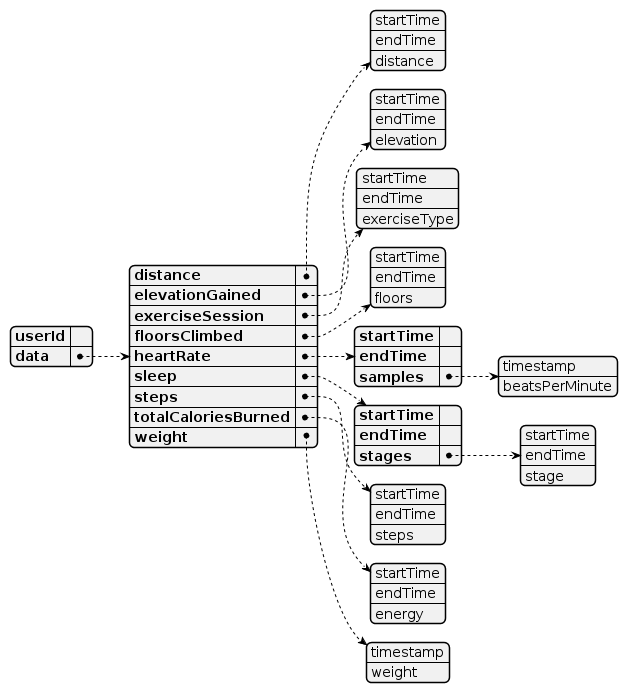
\includegraphics[width=0.75\textwidth]{figures/bd/Servidor user data.png}
    \caption[Diagrama colección datos usuario]{Diagrama colección datos usuario. Elaboración propia}
    \label{figure:disenio:diagrama_user_data}
\end{figure}

Diagrama colección cuestionarios diarios (\textit{daily questionnaires})

\begin{figure}[h]
    \centering
    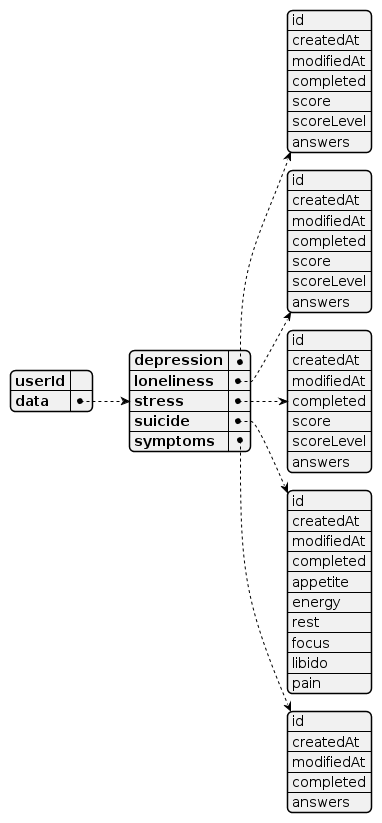
\includegraphics[width=0.33\textwidth]{figures/bd/Servidor daily questionnaires.png}
    \caption[Diagrama colección cuestionarios diarios]{Diagrama colección cuestionarios diarios. Elaboración propia}
    \label{figure:disenio:diagrama_daily}
\end{figure}

Diagrama colección cuestionarios puntuales(\textit{one off questionnaires})

\begin{figure}[h]
    \centering
    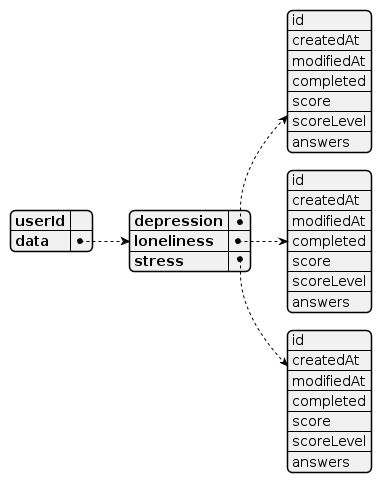
\includegraphics[width=0.33\textwidth]{figures/bd/Servidor one off questionnaires.png}
    \caption[Diagrama colección cuestionarios puntuales]{Diagrama colección cuestionarios puntuales. Elaboración propia}
    \label{figure:disenio:diagrama_one_off}
\end{figure}